\documentclass[runningheads]{llncs}
\usepackage{graphicx}

\begin{document}
\title{Question Hub}

\author{Group 22: Jakob Waibel \and Mouad Abuaisha \and Philipp Urban}

\institute{}
\maketitle              

\section{Introduction}

A group of independent computation devices connected by a network defines a
distributed system. In order for components to interact with each other and
schedule their actions so that users perceive the system as a single,
integrated computing facility, each host carries out computations and runs a
distribution middleware\cite{coulouris2005distributed}. Distributed systems
represent a significant advancement in computer science and IT. This is because
an increasing number of related tasks are getting scaled up and more
complicated and are beyond the capabilities of a single computer. Distributed
systems reduce the risks associated with a single point of failure and
therefore improve fault tolerance and reliability. Contemporary distributed
systems are typically built with near-real-time scalability in mind. This
allows for easy expansion and redistribution of computational resources, which
boosts efficiency and shortens completion times. The architecture of a 
distributed system focuses on the system as a whole and how its components are
distributed across several machines\cite{tanenbaum2007distributed}.
\newline
\newline
Question Hub is a distributed system for facilitating live Q\&A sessions.
Clients can ask and upvote questions anonymously in order to determine a
ranking on the site and hence allowing them to ask questions they would be too
afraid to ask otherwise. A lecturer can then answer questions according to that
ranking during a lecture. Each client can vote for a question exactly once.
Voting again removes the vote from the corresponding question.

\section{Project Requirements Analysis}

\subsubsection{Architecture Model}

The project should implement a client-server\cite{berson1996client} architecture equipped
with the ability to handle an arbitrary number of clients and servers. The
servers should represent control nodes that handle the data flow and application
state while ensuring the correct operation of the system. Each control nodes
maintains a separate copy of the application data. Multiple servers exist in
order to provide consistency and availability throughout the operation of the
application. Each user is utilizing a client instance in order to post or vote
for questions. Every action taken by a user will result in an update of the
application state that is then propagated back to the clients.

\subsubsection{Voting}

Voting shall be implemented in the form of a leader election algorithm. The leader
election algorithm should determine a server node that gets control
of the application state. If the leader fails, a new leader should be determined
immediately. 

\subsubsection{Dynamic Discovery of Hosts}

There can be an infinite number of clients and servers in the system. All nodes should
be able to discover the currently leading node via broadcast. The control node should then
notify the new node about the current network topology in order for the new node to be aware of the
current network topology going forward.

\subsubsection{Fault tolerance}

The system should still be functional, if single server instances fail. If a leader
fails, a new leader should be elected and take over the work from the previously
elected leader. Furthermore, the server nodes should regularly send heartbeat messages in order
to determine liveness of the server nodes and detect possible node failures.

\subsubsection{Ordered Reliable Multicast}

In order for the system to work in a consistent manner, it has to be guaranteed
that messages originating from the same host are delivered in a similar order
in which they were sent. In order to achieve this, first-in first-out reliable
ordered multicast should be implemented in order to guarantee that the heartbeat
messages can be processed currectly.

\subsection{Dynamic Discovery}

Host discovery works dynamically using broadcast messages.
Whenever a new node joins the network, it sends a broadcast message to notify
all other nodes about its presence.
\newline
\newline
In order to distinguish server and client
nodes, the servers utilize the \texttt{HELLO} OpCode, while the clients utilize the
\texttt{HELLO\_SERVER} OpCode. This is necessary since the different type of nodes are
handled differently i.e. a client node does not have to be taken in account for
possible future elections. By design, only the leader replies to \texttt{HELLO} and
\texttt{HELLO\_SERVER} messages utilizing unicast by sending a \texttt{HELLO\_REPLY} message
containing the current topology of the network as well as the application
state. This is possible since every node provides its unicast port as a field
inside of every broadcast message. This provides the benefit of automatically
announcing the current leader to the client as well as reducing the amount of
messages in the system.

\subsection{Fault Tolerance}

In order to achieve fault tolerance, the system needs to distinguish multiple
events that could lead to a failure. Liveness of the system is ensured by
server nodes regularly broadcasting heartbeat messages to each other utilizing a push-based approach. These
heartbeat messages ensure that every server node has a consistent topology of
the system and hence can initiate a leader election once a leader crashes.
A server is considered failed once a heartbeat that is normally sent every
second was not received for a total of two seconds for a particular node.
Once this event occurs, the node is removed from the topology and, if the node
was the leader, the remaining nodes initiate a new leader election.
If the failed node was not a leader, the system removes the node from the
topology and continues operation as normal.
\newline
\newline
If the server node reconnects at some point, it has to adhere to the
communication protol again by broadcasting a message of OpCode \texttt{HELLO}. 
Whenever a new node joins, it challenges the current leader by initiating a new
leader election.
\newline
\newline
Since the liveness of the system does not depend on client nodes, clients do not
have to broadcast regular heartbeat messages. Since the questions are anoymous
and are not less relevant when a client leaves, the application state does not
have to be adjusted after a client crashed.
\newline
\newline
By identifying clients based on their socket, a client cannot vote for questions
multiple times by reconnecting arbitrarily often, as long as it is using the same
socket. A reconnecting client has to retransmit the message with OpCode
\texttt{HELLO\_SERVER} just like the server.
\newline
\newline
In an attempt to handle byzantine failures, every operation a client wants to
perform is verified by the leading server instance before an operation is
executed. After the client sends a unicast message containing the action to the
leader and it has been verified, the server instance broadcasts the operation
to all nodes. This leads to clients receiving the most up to date information
in their respective frontend as well as replicating the application state to
all other server nodes in case the client crashes.


\subsection{Leader Election}

Electing a leader is performed using the Hirschberg-Sinclair algorithm which
resembles an algorithm for originally determinining the largest of $n$
processors that are arranged in a ring.
By utilizing the bidirectional capabilities of the Hirschberg-Sinclair
algorithm, a performance of $O(n\log{}n)$ is possible.\cite{hirschberg1980decentralized}
\newline
\newline
This algorithm was chosen since the number of participating nodes
does not need to be known at the beginning of the election.
In General, the algorithm sends a message around in a ring of all nodes.
Instead of comparing the size of processors, Question Hub is utilizing
random UUIDs that are generated upon node creation. If a node receives a
message from a node with a larger UUID, it just forwards that message onwards
to the next node in the ring. If a sender receives its own messages of OpCode 
\texttt{ELECTION\_VOTE} again i.e. it had the largest UUID of all nodes, it won the
election which will result in the winning node broadcasting a message of
OpCode \texttt{ELECTION\_REPLY}. 
\newline
\newline
In order to achieve the optimum number of messages
for the algorithm, the algorithm performs the election in rounds. The first
round sends a message with hop-distance 1 to the left and to the right in the
ring. In general, the hop distance can be described as sending messages a
distance of $2^i$ hops in phase $i$. When the final hop of a given phase $i$ is
reached, the receiver sends a message with OpCode \texttt{ELECTION\_REPLY} back in the
direction of the sender in order to notify the sender that the message received
its destination without being dropped due to a node having a higher UUID than
the sender. Hence, the sender can start another round of the election.
\newline
\newline
Whenever a new server node joins and receives a \texttt{HELLO\_SERVER}, it initiates a
new leader election in order to challenge the current maximum UUID in the
system in order to find out whether it should be the new leader.
When a node does not receive any messages of OpCode \texttt{HEARBEAT} for 2 seconds
and it is the only node in its node topology, it declares itself to be the
leader. Once a new leader was elected successfully, all nodes get a broadcast of
OpCode \texttt{ELECTION\_RESULT} In order to notify the nodes about the new leader.
Upon receiving this message, the clients switch their communication to the
new leader.

\subsection{Ordered Reliable Multicast}

Since the application logic is always processed through the leader and the
nodes get the application state from the leader at all times, ordered
reliable multicast is not required in this scenario.
\newline
\newline
Instead, the heartbeat messages are using first-in first-out multicast in order to ensure that the
servers receive the timestamps in right order. If messages arrived in a
different order, timestamps could vary so much, that a node could appear as if
it failed since the timestamp differs by more than two seconds. 
\newline
\newline
FIFO is implemented by inserting arriving heartbeat messages into a queue and
always delivering the message with the oldest heartbeat so that the heartbeat
messages arrive in the correct order.

\section{Architecture Design}

Question Hub is implemented using a client-server \cite{berson1996client} architecture
model with multiple servers and clients. The servers represent control nodess that handle the
data flow and application state while ensuring the correct operation of the system.
Each control nodes maintains a separate copy of the application data. Multiple servers exist
in order to provide consistency and availability throughout the operation of the
application. Each user is utilizing a client instance in order to post or vote for
questions. Every action taken by a user will result in an update of the application state.
\newline
\newline
The system can be scaled horizontally i.e. an arbitrary amount of $n$ server
nodes and $m$ client nodes can participate. A client consists out of a
frontend written using JavaScript and Vue as well as a middleware which exposes
an HTTP API for the frontend to work with. The middleware itself aquires its
data using socket communication with the currently leading server node. The
server nodes interface with the clients using sockets and messages containing
several different OpCodes e.g. \texttt{HELLO}, \texttt{VOTE\_REQUEST} or \texttt{ELECTION\_RESULT}.
In order to still deploy the client as one component, the subcomponents are
containerized while still using the network of the host. By following this
approach, the system can still be operated in a distributed manner. 

\begin{figure}
    \centering
    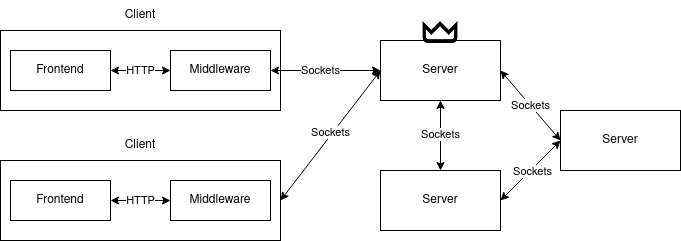
\includegraphics[width=\linewidth]{question_hub_architecture_final.drawio.png}
    \caption{System Design Architecture Diagram}
    \label{fig:enter-label}
\end{figure}

\section{Implementation}

The system is comprised out of multiple components: The frontend, the
middleware and the server. The frontend is implemented using JavaScript and
Vue. The frontend fetches its data from a REST API that is exposed by the
middleware. It provides a minimal set of endpoints that suffice to perform the
business logic of the system: 

\begin{itemize}
    \item \textbf{\texttt{[GET]}}: \texttt{/api/get} fetches the application data
    \item \textbf{\texttt{[POST]}}: \texttt{/api/vote} votes for a question by providing the question id
    \item \textbf{\texttt{[POST]}}: \texttt{/api/question} post a new question
\end{itemize}

Since the whole application data is fetched from the middleware whenever an
update is aquired and the middleware is running on the same node as the
frontend, additional API calls are not necessary.
\newline
\newline
The clients communicate with the servers using sockets. The server and the
client middleware are implemented using Python. The REST API is implemented
using Python's flask library. Multiple threads are utilized to listen on
multiple channels simultaneously. One thread listens for broad- and multicast
messages, one thread listens for unicast messages and one is exclusively
handling heartbeat messages.
\newline
\newline
The API between the client and the server adheres to the following OpCodes:

\begin{itemize}
    \item \textbf{\texttt{HELLO\_SERVER}} announces the clients presence to the server 
    \item \textbf{\texttt{HELLO\_REPLY}} acknowledges the announcement and contains the current application state for the client
    \item \textbf{\texttt{QUESTION\_REQUEST}} sends a question request to the server
    \item \textbf{\texttt{QUESTION}} acknowledges the question and broadcasts it to all nodes
    \item \textbf{\texttt{VOTE\_REQUEST}} sends a vote request containing the corresponding question id to the server
    \item \textbf{\texttt{VOTE}} acknowledges the vote and broadcasts it to all nodes
    \item \textbf{\texttt{ELECTION\_RESULT}} broadcasts the election result to all nodes
\end{itemize}

The communication between servers requires some additional message types in
order to address the leader election and fault tolerance:

\begin{itemize}
    \item \textbf{\texttt{HELLO}} to announce the servers presence
    \item \textbf{\texttt{HEARTBEAT}} to send a liveness probe to the other server nodes
    \item \textbf{\texttt{ELECTION\_VOTE}} to send a vote for a leader election
    \item \textbf{\texttt{ELECTION\_REPLY}} to send a reply back to the sender of the vote
    \item \textbf{\texttt{APPLICATION\_STATE}} to send the application state to a new server node
\end{itemize}

Architecturewise, the code is seperated into multiple components representing
the several layers on the client and server-side. Each node contains a
\texttt{ControlPlane} that contains the management of the topology of the
network as well as the representation of the nodes as a ring for the leader
election. Networking is handled using \texttt{Message}s that are responsible
for composing, marshalling, unmarshalling and sending messages of several
OpCodes. Messages are transmitted utilizing JavaScript Object Notation (\texttt{JSON}).
This allows for conveniently marshalling and unmarshalling messages and access
fields across multiple languages. Leader elections also compose a separate component, namely \texttt{Election}
that is responsible for handling the election process.

\section{Discussion and Conclusion}

Question Hub forms a distributed system implementing several basic concepts e.g. leader election, dynamic discovery of hosts, fault tolerance.
However, if the system would be utilized in a production environment, there are several points that could be improved. The current implementation utilizes
a random UUID in order to determine a leader. Since the Hirschberg-Sinclair algorithms aims at determining a leader based on some metric like processor size or remaining disk-capacity.
In a production environment, this metric could be useful and actually affect  the performance of a large-scale distributed system. Furthermore, additional ways of handling node failures might be useful for a production-grade system. Currently, only node crashes and invalid application state transitions are handled properly. 
However, Question Hub provides a solid implementation for the scale of this project, implementing all of the set requirements.

\begin{thebibliography}{8}
    \bibitem{lamport2019byzantine}Lamport, L., Shostak, R. \& Pease, M. The Byzantine generals problem. {\em Concurrency: The Works Of Leslie Lamport}. pp. 203-226 (2019)
    \bibitem{hirschberg1980decentralized}Hirschberg, D. \& Sinclair, J. Decentralized extrema-finding in circular configurations of processors. {\em Communications Of The ACM}. \textbf{23}, 627-628 (1980)
    \bibitem{dommel2000orderedmulticast}Dommel, H.-P. and Garcia-Luna-Aceves, J.J. Ordered end-to-end multicast for distributed multimedia systems {\em Proceedings of the 33rd Annual Hawaii International Conference on System Sciences} pp. 10 (2000)
    \bibitem{coulouris2005distributed}Coulouris, G., Dollimore, J. \& Kindberg, T. Distributed systems: concepts and design. (pearson education,2005)
    \bibitem{tanenbaum2007distributed}Tanenbaum, A. Distributed systems principles and paradigms.  (2007)
    \bibitem{berson1996client} Berson, A. Client/Server Architecture 1996
    \bibitem{ongaro2014search}Ongaro, D. \& Ousterhout, J. In search of an understandable consensus algorithm. {\em 2014 USENIX Annual Technical Conference (USENIX ATC 14)}. pp. 305-319 (2014)
    \bibitem{lamport2019part}Lamport, L. The part-time parliament. {\em Concurrency: The Works Of Leslie Lamport}. pp. 277-317 (2019)
\end{thebibliography}
\end{document}
